\section{Methodology (1 page)}
\label{sec:methods}
\subsection{Crawling infrastructure}
We injest records from OpenPhish, PhishTank, APWG, and PhishingDB. For a portion of the time perioud we also recive pages from a dataset of mobile specific phishing pages from Nahapetyan \etal{} and URLScan.

We crawl the pages every 2 hours, using a automated crawler powered by the VisibleV8 patches.

To establish a data set with ground truth labels, we use KitPhisher\todocite{KitPhisher} to extract phishing kits for pages where the malicious actor accidently left the kit on the server.

\begin{figure}[t]
    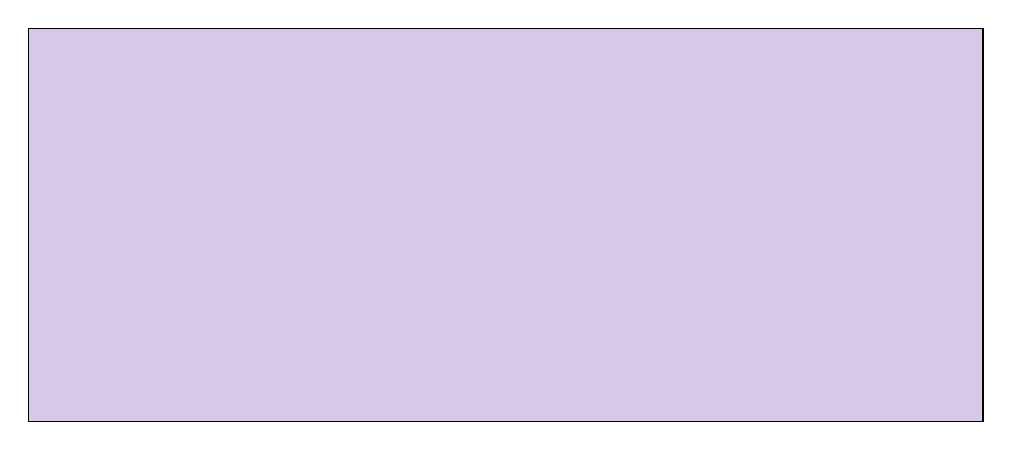
\begin{tikzpicture}
      \node[draw, fill=RoyalPurple!20, minimum width=\columnwidth, minimum height=5cm] {};
    \end{tikzpicture}
    \caption{Crawling infrastructure}
    \label{fig:infra}
    \Description["TODO: "]{"TODO"}
  \end{figure}
\subsection{Data enrichment}
\DraftToDo{isolating First party scripts, browser-specific APIs w/ IDL, MDN categories}

We use the VisibleV8\todocite{VV8} patches to monitor the browser API calls, and property accesses. We use the Chrome IDL data to filter out the browser API calls from the noise.

When we need further aggregation of the type of APIs we see, we use the MDN categories\todocite{MDN} to classify the APIs into categories. We obtain these categories by processing the markdown files in the MDN repository.

In order to cut through the noise of cloacked pages and included third party scripts like google analytics, which prior work shows and we confirm is used by phishing pages, we isolate API sets that are executed by first party scripts (from now on called first party API set). To do this, we establish the root domian to be the domain that was submitted to the feeds, and the origin to be the domain that the script is loaded from. We consider a script first party only if it is loaded from the same domain that we aquared from our feeds (root domain). 
\DraftToDo{explain how does this cut through the noise of cloacking}

To establish which APIs are related to client-side cloacking as discussed by Zhang \etal{}\todocite{crawlphish}, we both manually create a list of APIs that fall under the categories described in the paper. As well as query only the APIs that were listed in the paper.
\DraftToDo{Explain the difference\ldots{} Basically there is more APIs if you consider User-interaction as any click related stuff, and Fingerprint as ALL known FP apis}

\begin{table}[t]
    
    \caption{Manual criteria to identify cloaking behavior established by Zhang \etal{}}
    \resizebox{\columnwidth}{!}{%\centering
    \begin{tabular}{cl}
        \textbf{Cloaking Category} & \multicolumn{1}{c}{\textbf{Required API calls}}                                                                                  \\ \hline
        User Interaction           & \begin{tabular}[c]{@{}l@{}}Any permission requesting API call\\ FilePicker API calls \\ HTMLElement event listeners\end{tabular} \\ \hline
        Fingerprinting             & \begin{tabular}[c]{@{}l@{}}HTMLDocument.cookie \\ HTMLDocument.referrer\\ Navigator.userAgent\end{tabular}                               \\ \hline
        Bot Behavior               & \begin{tabular}[c]{@{}l@{}}Crypto.getRandomBytes\footnote{Since Math.random is a javascript builtin function, VisibleV8 does not have visibility into it's execution}\\ Window.setTimeout + Performance.now\end{tabular}                          
        \end{tabular}
    }
\label{tab:behaviorcategories}
\end{table}
\subsection{Identifying trends }
For anomoly detection, we use rapture\todocite{ruptures} to detect changepoints in the time series of API calls. We use the L1 cost function with a linearly penalized segmentation algorithm to find segments based on the mean deviation.
\DraftToDo{Go into detail how do we evaluate this. Also\ldots{} figure out how we are going to evaluate this.}
VisibleV8 will de-duplicate the same script loaded by multiple pages via the sha3 hash of the script. In order to establish if scripts are having non-deterministic behavior, we pull the set of APIs that are executed by the script, and compare the set of APIs executed by the same script on different pages. We use the Jaccard index to establish the simularity between the sets of APIs.

\subsection{Identifying kits}

The core hypothesis of this work is that simularity in the browser API execution mean that the pages originate from the same phishing kit. To establish this simularity, we use the Jaccard index on the set of APIs that first party scripts execute. 

We use HDBScan, with a minimum cluster size of 10, to cluster the pages based on the Jaccard index. We then use the ground truth labels from KitPhisher to evaluate the clustering. When ground truth is available, we use Fowlkes-Mallows Index (geometric mean between percision and recall)\todocite{Normalised Clustering Accuracy: An Asymmetric External Cluster Validity Measure}, and V-measure to evaluate the clustering.
\DraftToDo{Go into detail why V-measure and what it can tell us}

In cases when we do not have ground truth, we use the silhouette score to evaluate the clustering.
\DraftToDo{Go into detail why}
\DraftToDo{Davies-Bouldin Index?}

% \subsection{Phishing Feeds and crawling}

% We monitor Phishtank\todocite{PhishTank}, OpenPhish\todocite{OpenPhish}, PhishingDB\todocite{PhishingDB}, APWG\todocite{APWG}, and list of phishing urls from sms gateways\todocite{us or just drop this?}.

% We crawled the pages ever 2 hours, using a automated crawler powered by the VisibleV8\todocite{VV8} patches.

% The crawler gives us insight into all javascript method calls, and property accesses, that we filter down to browser API call using the chrome idl data.

% Our data collecting has a diverse set of techniques just at the deployment stage! docs has power-points that you have to click through to get to the page, we see a lot of blogspot, and scripts are hosted all over the place, including other phishing pages.

% \todowrite{Table of top hostnames for scripts...}
% \subsection{Data post processing}

% VisibleV8 comes with built-in post-processors that can isolate browser API calls per origin that they are called in and the URL of the script executing (in the case of a script embedded in the HTML, the origin of is the script URL).

% \subsection{Analysis}

% The provided log processors can handle isolating the browser APIs calls per origin, however, in this subsection, we describe everything else we did to isolate trends within our dataset.

% \subsubsection{MDN APIs}

% Mozilla Developer Center's Web Docs \todocite{MDN}, is documentation on different browser APIs that can be used in the modern web. The documentation breaks down the APIs into \mdncategorytotal{} categories. They also label if an API category is classified as experimental, for example, the Barcode Detection API.

% \subsubsection{Classifying Temporal behavior}

% We describe API behavior as an increase, decrease, dip (a decrease followed by an increase), or a spike (an increase followed by a decrease).

% We first isolate out 3,978 browser APIs that show up at least in 100 web pages, we use change point detection to identify the different sections within a time series of each API. For change point detection use use ruptures\todocite{ruptures}. We use an L1 cost function along with a Linearly penalized segmentation algorithm to find the median's segmentation point of a deviation.\

% To filter out noise results, we only consider APIs with at least 2 but no more than 5 segments.

% \subsubsection{Cloaking identification}

% We manually create a list of APIs that can be used to redirect the user using client-side javascript.

% \subsubsection{First Party / Third Party identification}

% A script can be third party relative to the origin it is being loaded, or the root domain (the domain submitted). Since scripts first party to the origin can still be 3rd party scripts that are loaded in an iframe, and to minimize pollution from server-side cloaking, we consider a script first party only if it is loaded from the same domain that we aquared from our feeds.

% % \subsubsection{Kit identification}
% \subsection{Phishing behavior API categories}

% \begin{table}[t]
    
    \caption{Manual criteria to identify cloaking behavior established by Zhang \etal{}}
    \resizebox{\columnwidth}{!}{%\centering
    \begin{tabular}{cl}
        \textbf{Cloaking Category} & \multicolumn{1}{c}{\textbf{Required API calls}}                                                                                  \\ \hline
        User Interaction           & \begin{tabular}[c]{@{}l@{}}Any permission requesting API call\\ FilePicker API calls \\ HTMLElement event listeners\end{tabular} \\ \hline
        Fingerprinting             & \begin{tabular}[c]{@{}l@{}}HTMLDocument.cookie \\ HTMLDocument.referrer\\ Navigator.userAgent\end{tabular}                               \\ \hline
        Bot Behavior               & \begin{tabular}[c]{@{}l@{}}Crypto.getRandomBytes\footnote{Since Math.random is a javascript builtin function, VisibleV8 does not have visibility into it's execution}\\ Window.setTimeout + Performance.now\end{tabular}                          
        \end{tabular}
    }
\label{tab:behaviorcategories}
\end{table}

% We hand created a criteria for API to match the categories of cloaking behavior classified in Crawlphish by Zhang. \etal{}\todocite{crawlphish}. We describe the criteria for every categories for Table-\ref{tab:behaviorcategories}.
